\documentclass[12pt, letterpaper]{article}
\usepackage{xcolor}
\usepackage{graphicx}
\usepackage{hyperref}
\usepackage{tabularx}
\usepackage{pgfplots}
\pgfplotsset{compat=1.18}
\usepackage{csvsimple}
\usepackage[utf8]{inputenc}
\usepackage{listings}
\usepackage{dirtree}
\usepackage{floatrow}
\usepackage{subfigure}


\definecolor{codegreen}{rgb}{0,0.6,0}
\definecolor{codegray}{rgb}{0.5,0.5,0.5}
\definecolor{codepurple}{rgb}{0.58,0,0.82}
\definecolor{backcolour}{rgb}{0.95,0.95,0.92}
\lstdefinestyle{mystyle}{
    backgroundcolor=\color{backcolour},
    commentstyle=\color{codegreen},
    keywordstyle=\color{magenta},
    numberstyle=\tiny\color{codegray},
    stringstyle=\color{codepurple},
    basicstyle=\ttfamily\footnotesize,
    breakatwhitespace=false,
    breaklines=true,
    captionpos=b,
    keepspaces=true,
    numbers=left,
    numbersep=5pt,
    showspaces=false,
    showstringspaces=false,
    showtabs=false,
    tabsize=2
}
\lstset{style=mystyle}

\def\timestamp{2023-06-02-10-27-57}
\def\rootDir{../..}
\def\csvStats{\rootDir/stats/stats_\timestamp.csv}
\def\pngStats{\rootDir/stats/plot_\timestamp.png}

\hypersetup{
    colorlinks=true,
    linkcolor=blue,
    filecolor=magenta,
    urlcolor=cyan,
    pdftitle={Overleaf Example},
    pdfpagemode=FullScreen,
}
\pgfplotsset{width=10cm}

\title{NLP Twitter Analysis}
\author{Hamed Feizabadi}
\date{\today}

\begin{document}
    \thisfloatsetup{%
        objectset=raggedright,
    }
    \maketitle
    \tableofcontents
    \newpage


    \section{Introduction}\label{sec:introduction}
    This is the final report for the NLP course project. In this project we have collected tweets from Twitter and labeled them using ChatGPT model. Then we have augmented the data using GPT-3.5-turbo model. After that we have trained a classifier using the augmented data and evaluated the results.

    Word2vec, tokenizer and language model and other stuffs also have been trained on the collected data, which we will discuss in the following sections.


    \section{Repository}\label{sec:repository}
    You can access the source code of this project at \url{https://github.com/hamedhf/nlp_twitter_analysis}

    \section{Requirements}\label{sec:requirements}
    If you have a GPU(especially Nvidia) then you are good to go and can run project locally, as we did. Otherwise you can use Google Colab to run the project. For that purpose you need to clone the github repo inside colab and run the commands provided with main.py file. These commands are also provided in the README.md file of the repository.

    \section{Installation}\label{sec:installation}
    You should create a file named "users.csv" inside src folder which contains the Twitter username, University name an Actual name of the users you wish to analyze.

    Furthermore installation instructions are provided in the README.md file of the repository.


    \section{Project Structure}\label{sec:project-structure}
    \begin{figure}[H]
        \dirtree{%
            .1 rootfolder.
            .2 data.
            .3 raw.
            .3 clean.
            .3 wordbroken.
            .3 sentencebroken.
            .3 augment.
            .3 split.\dotfill\begin{minipage}[t]{5cm}
                                 parsbert finetune data
            \end{minipage}.
            .3 language\_model.\dotfill\begin{minipage}[t]{5cm}
                                           gpt2-fa finetune data
            \end{minipage}.
            .2 logs.\dotfill\begin{minipage}[t]{5cm}
                                all project logs
            \end{minipage}.
            .2 models.
            .3 gpt2.\dotfill\begin{minipage}[t]{5cm}
                                gpt2 farsi model
            \end{minipage}.
            .3 parsbert.\dotfill\begin{minipage}[t]{5cm}
                                    parsbert model
            \end{minipage}.
            .3 word2vec.\dotfill\begin{minipage}[t]{5cm}
                                    word2vec model
            \end{minipage}.
            .2 src.
            .3 latex.\dotfill\begin{minipage}[t]{5cm}
                                 latex source files
            \end{minipage}.
            .3 main.py.\dotfill\begin{minipage}[t]{5cm}
                                   main script for running commands
            \end{minipage}.
            .3 utils.
            .4 augment.py.\dotfill\begin{minipage}[t]{5cm}
                                      augment data using gpt-3.5-turbo
            \end{minipage}.
            .4 clean.py.\dotfill\begin{minipage}[t]{5cm}
                                    clean data
            \end{minipage}.
            .4 crawl.py.\dotfill\begin{minipage}[t]{5cm}
                                    crawl data from twitter
            \end{minipage}.
            .4 label.py.\dotfill\begin{minipage}[t]{5cm}
                                    label data using chatgpt
            \end{minipage}.
            .4 split.py.\dotfill\begin{minipage}[t]{5cm}
                                    split data into train, test and validation
            \end{minipage}.
            .4 constants.py.\dotfill\begin{minipage}[t]{5cm}
                                        project constants and configurations
            \end{minipage}.
            .4 word2vec.py.\dotfill\begin{minipage}[t]{5cm}
                                       train word2vec model
            \end{minipage}.
            .4 gpt2.py.\dotfill\begin{minipage}[t]{5cm}
                                   train gpt2 model
            \end{minipage}.
            .4 parsbert.py.\dotfill\begin{minipage}[t]{5cm}
                                       train parsbert model
            \end{minipage}.
            .4 ....
        }
        \caption{Project Tree}
    \end{figure}


    \section{Data Collection}\label{sec:data-collection}
    We used selenium $>=$ 4.6.0 for collecting data from Twitter. This tool helps us to bring up an actual browser and navigate through the pages. Note that you should have Chrome installed on your system for this to work. Then you can simply install other dependencies form pyproject.toml file using poetry or other package managers.
    The crawler script reads the users.csv file and for each user, it navigates to the user's profile and collects the tweets. The tweets are stored in a file named unlabeled.db inside data\slash raw folder. Then labeling script uses this and with the help of ChatGPT model, it generates the labels for each tweet and stores them in data\slash raw\slash labeled-run-date.csv file.


    \section{Data Format}\label{sec:data-format}
    The data is stored in a csv file with the following format:\\ tweet\_time, tweet\_owner, tweet\_text, owner\_university, owner\_name, label.
    We use tweet\_time, tweet\_owner as unique identifiers for each tweet. The tweet\_owner is Twitter username of the owner. The tweet\_text is the actual text of the tweet. owner\_university and owner\_name are the university and actual name of the tweet owner. The label is the generated label for the tweet.


    \section{Data Preprocessing}\label{sec:data-preprocessing}
    We have splitted data with three criteria: split by sentence with hazm sentence tokenizer, split by word with hazm word tokenizer, split by word with hazm lemmatizer.

    For cleaning the data, we used the following steps: remove emojis, remove urls, remove hashtags, remove mentions, remove numbers, remove punctuations. We used the hazm, cleantext and nltk libraries for this purpose.


    \section{Labeling}\label{sec:labeling}
    We give label to the whole tweet using ChatGPT. For more info about labeling see the src\slash utils\slash label.py file. You can also see the labels in src\slash utils\slash constants.py file.


    \section{Statistics}\label{sec:statistics}
    \csvautotabular{\csvStats}
    \begin{center}
        \includegraphics[width=1\textwidth]{\pngStats}
    \end{center}


    \section{Augmenting Data}\label{sec:augmenting-data}
    For this part to work you need to sign up for an account at \url{https://platform.openai.com} and provide your openai api key in .env file. Then you can run the augment-data command.

    The augmentation script takes a cleaned csv file as input and counts how many tweet we have for each label. Then it will fix the imbalance of the data by generating new tweets for the labels with less tweets. The generated tweets are stored in data\slash augment folder.

    You can see the implementation detail of the augmentation script in src\slash utils\slash augment.py file. We have used gpt-3.5-turbo model for this purpose and the given prompt is like this:
    \begin{lstlisting}[language=Python]
    import openai
    label = "home_and_garden"
    temperature = 0.6
    system_message = "Generate an informal Persian tweet about the given topic without any hashtags, mentions, links, or emojis."  # noqa
    messages = [
        {
            "role": "system",
            "content": system_message
        },
        {"role": "user", "content": f"topic: {label}"}
    ]
    response = openai.ChatCompletion.create(
        model="gpt-3.5-turbo",
        messages=messages,
        temperature=temperature,
        timeout=120
    )
    \end{lstlisting}
    Temperature is a parameter that controls the randomness of the generated text. The higher the temperature, the more random the text. The lower the temperature, the more predictable the text. We have used 0.6 for this parameter and it is random enough for our purpose and if we increase it will take much more time to generate the text and this is not practical for our purpose.

    Using this approach we have doubled our total data size and each label has at least 200 tweets. It is worth mentioning that because of openai api rate limit, it took us about \textbf{2 and a half days} to generate the data.

    \subsection{Generated Tweets}\label{subsec:generated-tweets}
    Some of the generated tweets:
    \begin{center}
        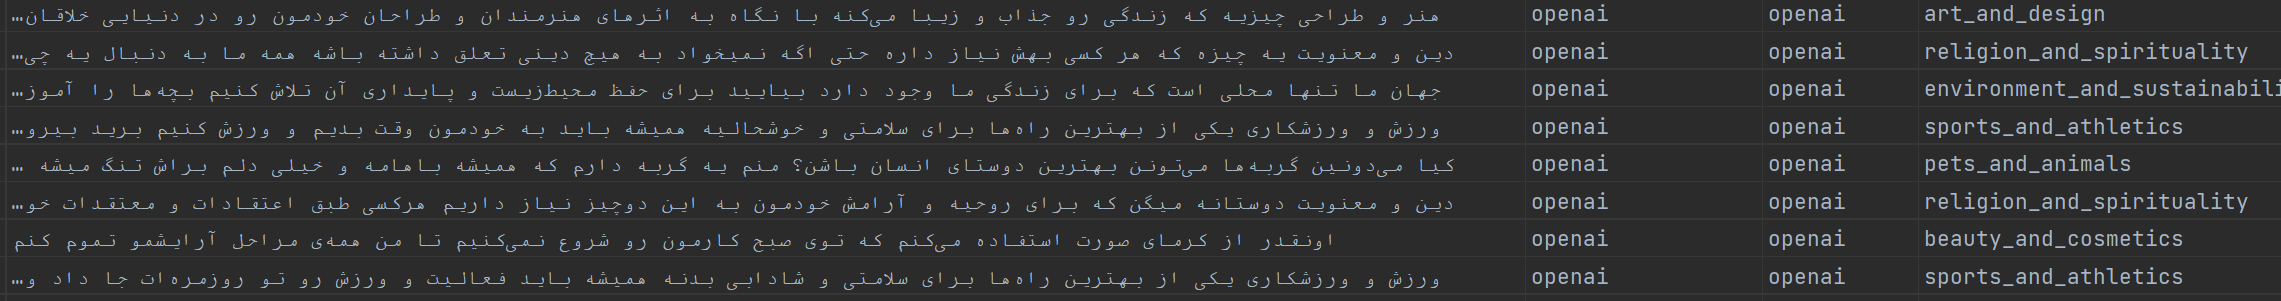
\includegraphics[width=1\textwidth]{images/generated_tweets.png}
    \end{center}

    \subsection{Augmented Data Statistics}\label{subsec:augmented-data-statistics}
    \begin{center}
        \csvreader[tabular=|c|c|c|,
        table head=\hline & label & tweet count\\ \hline,
        late after line=\\ \hline
        ]{\rootDir/stats/augmented_counts.csv}{}{
            \thecsvrow & \csvcoli & \csvcolii
        }
    \end{center}

    \section{Word2Vec}\label{sec:word2vec}
    We used gensim library for training skipgram word2vec model because it is easy to use and fast. The implementation is in src\slash utils\slash word2vec.py file.

    All ot the available commands are listed in \textbf{ReadME.md} file. Here we explain some of them.
    \subsection{Training}\label{subsec:training}
    This command trains word2vec for a specific label.
    \begin{lstlisting}[language=bash]
    python src/main.py train-word2vec-label path-to-augmented-csv home_and_garden
    \end{lstlisting}

    This command trains word2vec for some preselected labels.
    \begin{lstlisting}[language=bash]
    python src/main.py train-word2vec-preselected path-to-augmented-csv
    \end{lstlisting}

    This command trains word2vec for all labels.
    \begin{lstlisting}[language=bash]
    python src/main.py train-word2vec-all path-to-augmented-csv
    \end{lstlisting}
    Each model is saved in a models\slash word2vec\slash label.npy file.

    \subsection{Evaluation}\label{subsec:evaluation}
    Let's find that in topic of home\_and\_ garden, which words are similar to the Persian word for home (khaneh).
    \begin{center}
        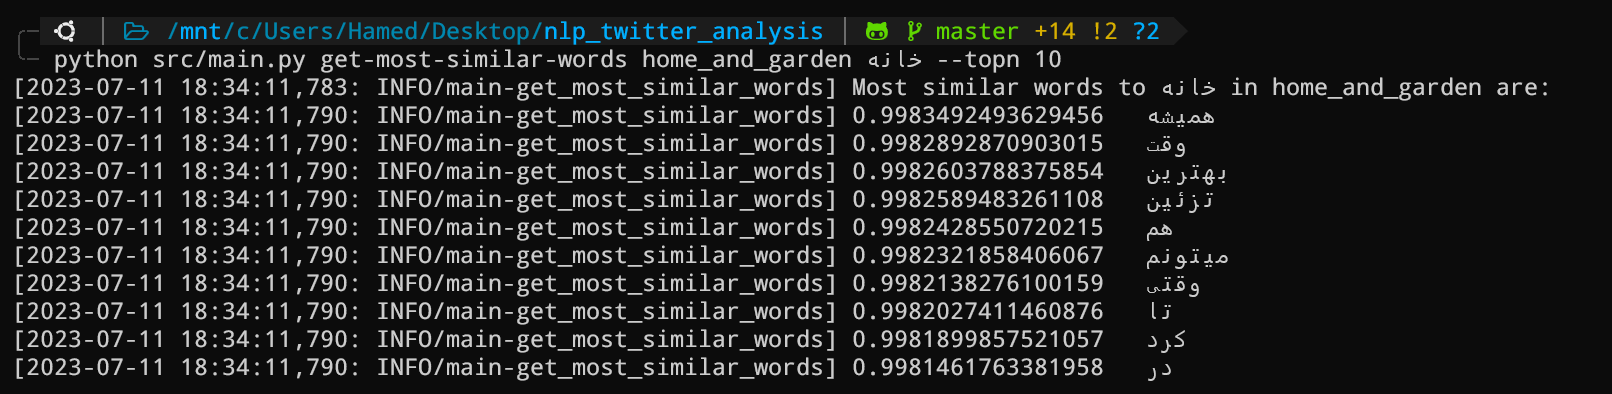
\includegraphics[width=1\textwidth]{\rootDir/src/latex/images/home_and_garden.png}
    \end{center}

    Some of the similarity results are shown in the following image. We use cosine similarity for measuring the similarity between two words. The higher the similarity, the more similar the words are.
    \begin{center}
        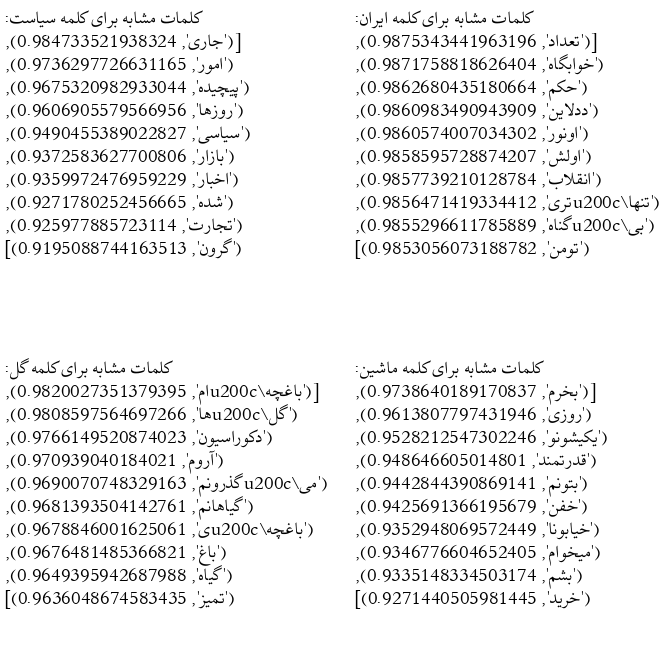
\includegraphics[width=1\textwidth]{\rootDir/stats/word2vec_similar.png}
    \end{center}

    \section{Language Model}\label{sec:language-model}
    We used huggingface transformers library for training the language model. The implementation is in src\slash utils\slash gpt2.py file. We used HooshvareLab/gpt2-fa model for this purpose. The model is trained on huge Persian corpus and it is available at \url{https://huggingface.co/HooshvareLab/gpt2-fa}. Use of pretained model helps us gain better results with less data.
    
    \subsection{Fine Tuning}\label{subsec:fine-tuning}
    The below command shows how to fine tune the model for a specific label. The script will check for dataset in data\slash languagemodel and if it is not available, it will create it using the augmented data. Then it will fine tune the model for the given label and save the model in models\slash gpt2\slash label folder.
    \begin{center}
        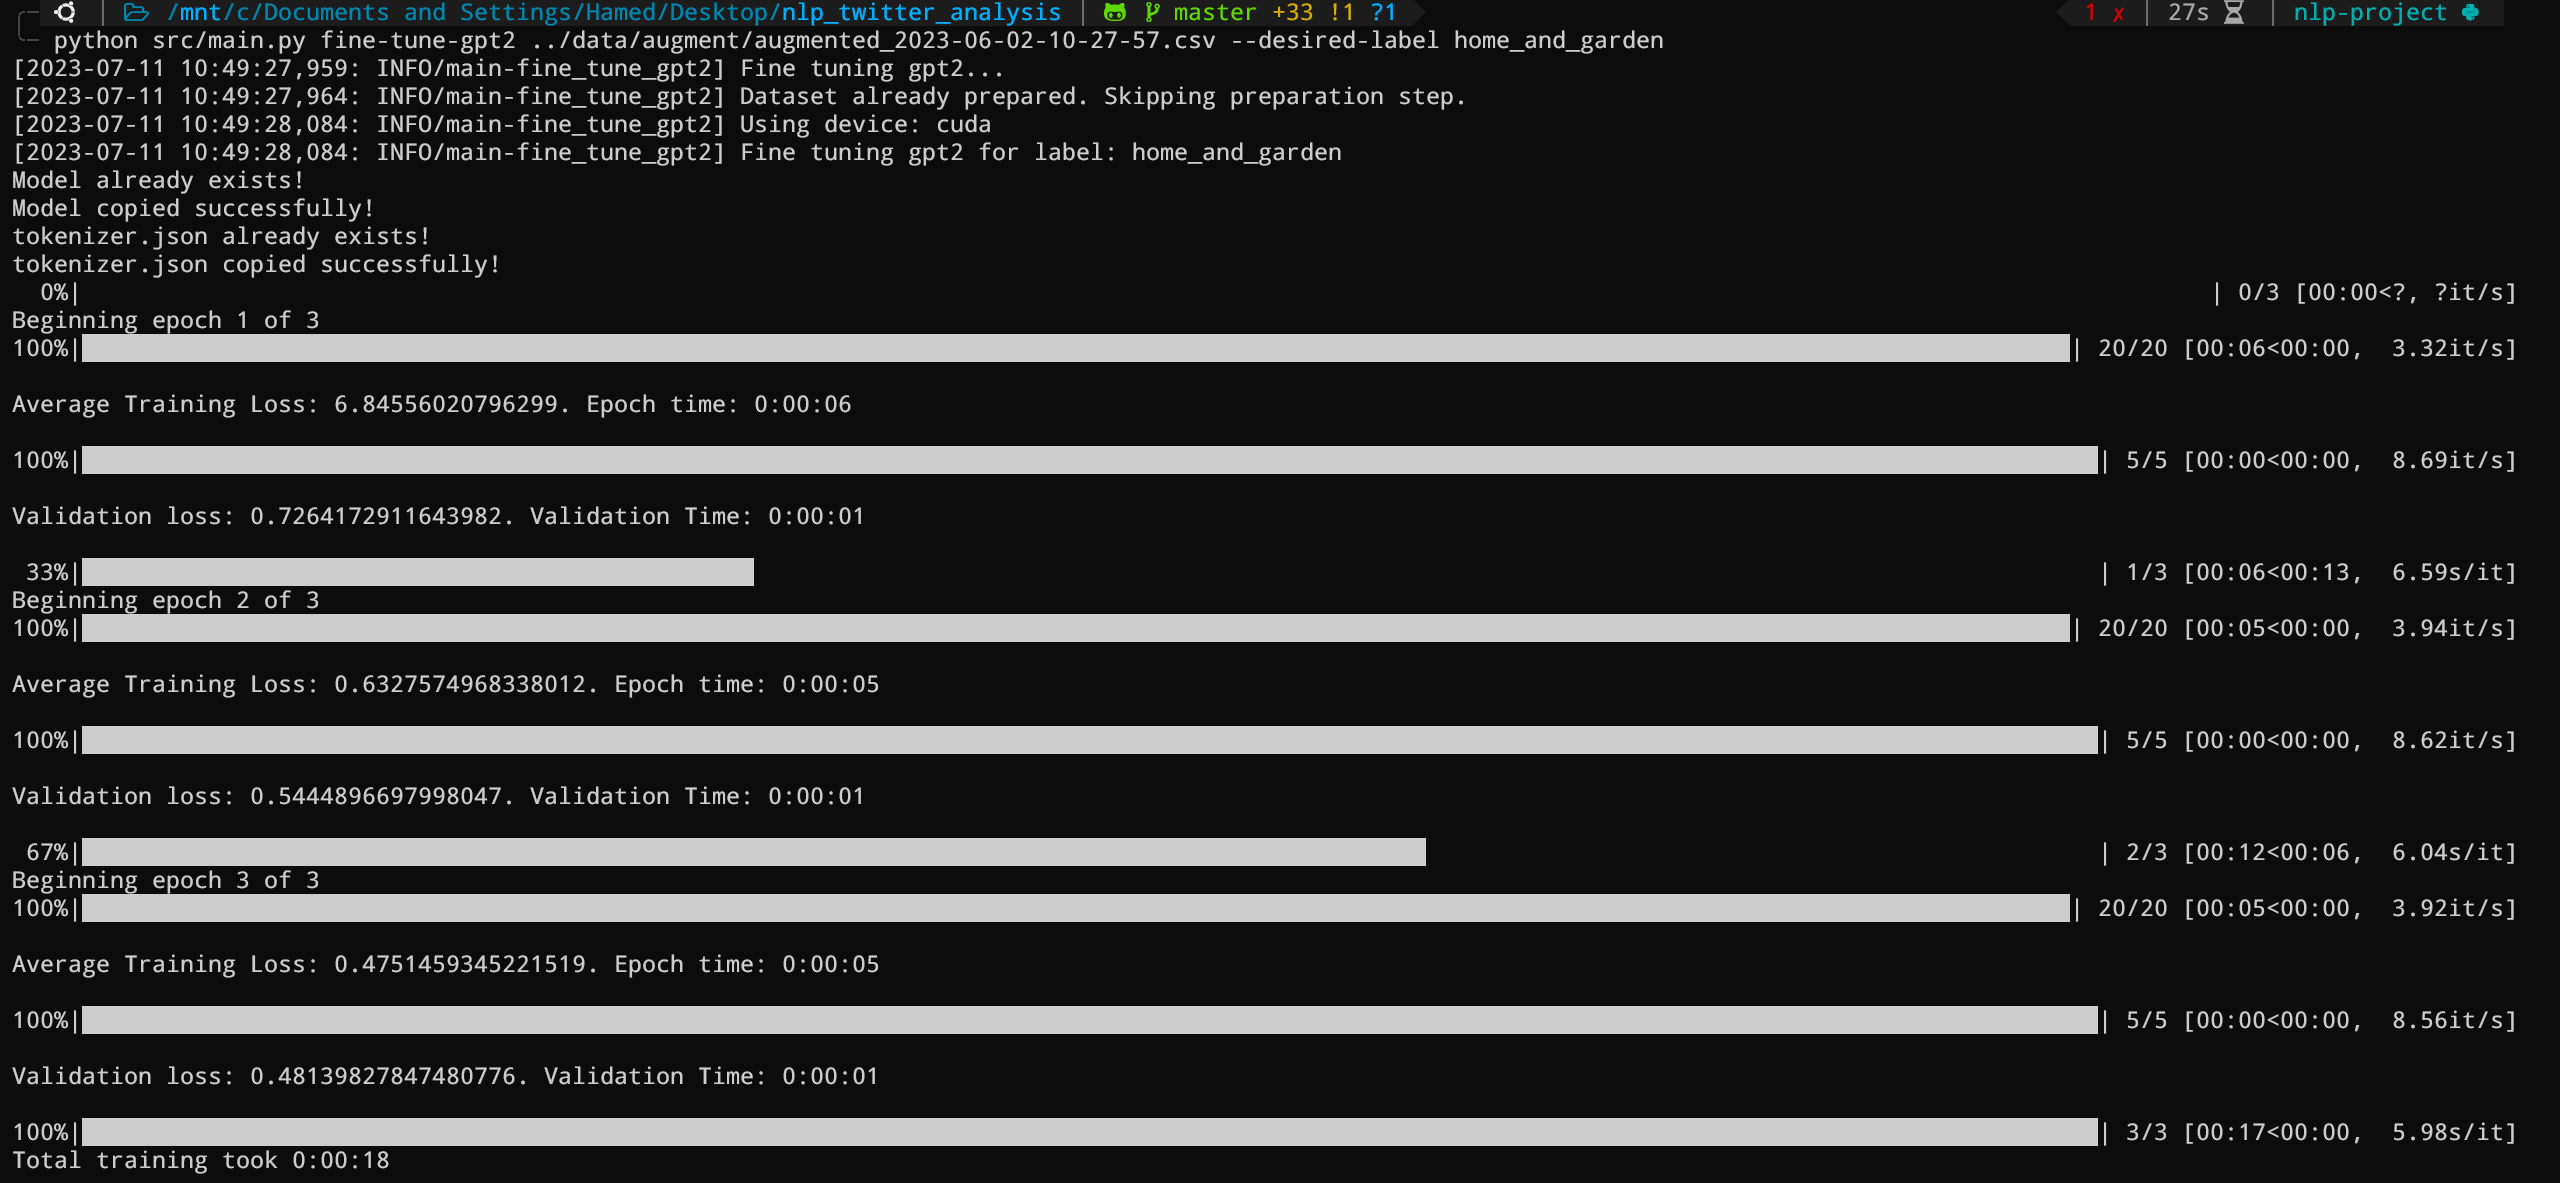
\includegraphics[width=1\textwidth]{\rootDir/src/latex/images/train-gpt2.png}
    \end{center}

    \subsubsection{Training and Validation Loss}\label{subsubsec:training-and-validation-loss}
    Following image shows the training and validation loss for some of the preselected labels, which you can see the list of them in src\slash utils\slash constants.py file. Also you can fine tune the model for them too. If you provide a label then it will be fine tuned for that label, otherwise it will be fine tuned for all of the preselected labels.
    \begin{figure}[H]
        \centering
        \subfigure[education\_and\_learning]{
        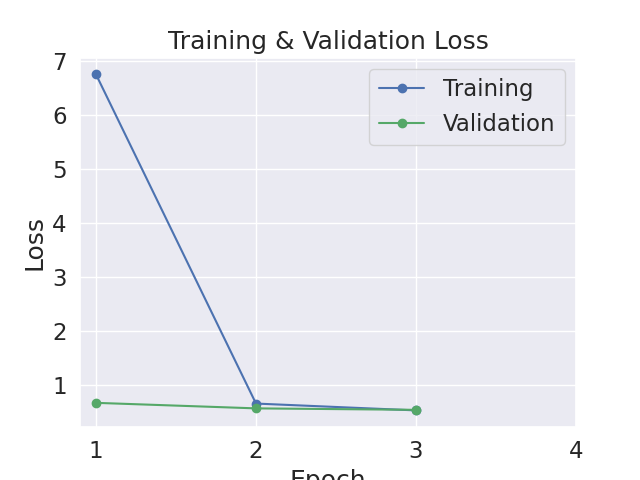
\includegraphics[width=0.4\textwidth]{\rootDir/stats/plot_gpt2_finetuning_education_and_learning.png}
        }
        \subfigure[environment\_and\_sustainability]{
        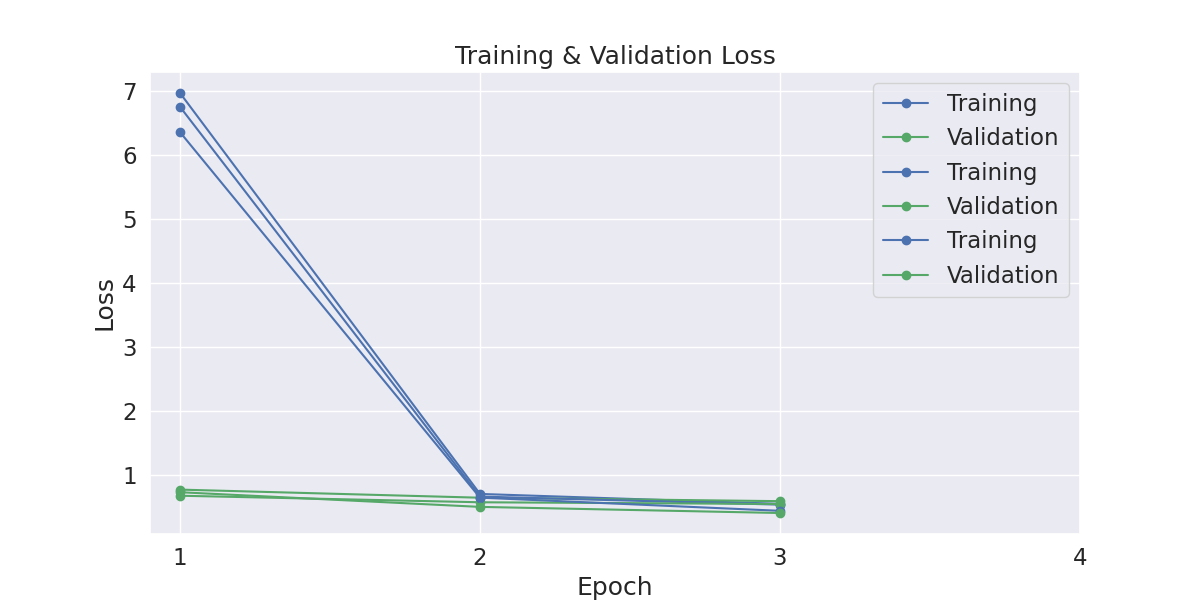
\includegraphics[width=0.4\textwidth]{\rootDir/stats/plot_gpt2_finetuning_environment_and_sustainability.png}
        }
        
        \subfigure[home\_and\_garden]{
        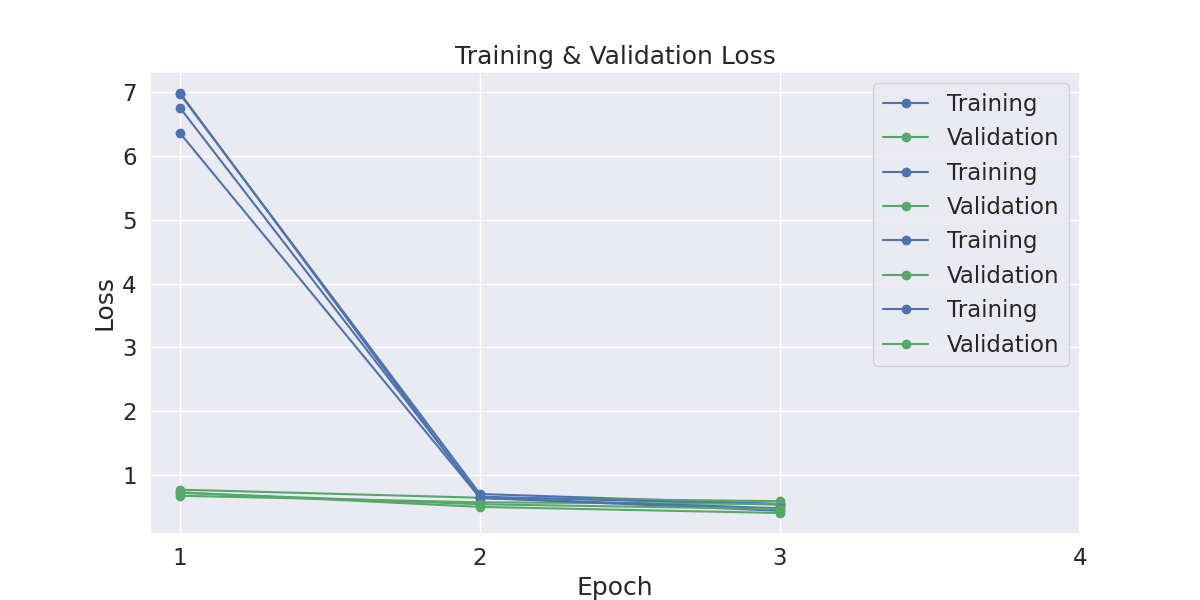
\includegraphics[width=0.4\textwidth]{\rootDir/stats/plot_gpt2_finetuning_home_and_garden.png}
        }
    \end{figure}

    \begin{figure}[H]
        \subfigure[politics\_and\_current\_affairs]{
        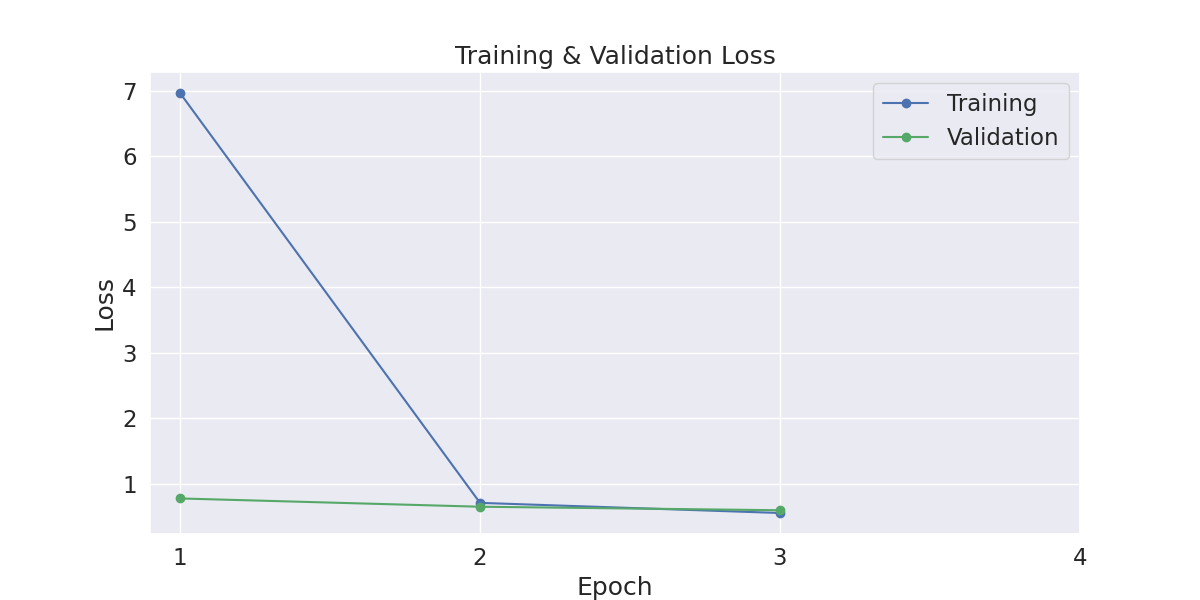
\includegraphics[width=0.4\textwidth]{\rootDir/stats/plot_gpt2_finetuning_politics_and_current_affairs.png}
        }

        \subfigure[weather\_and\_seasons]{
        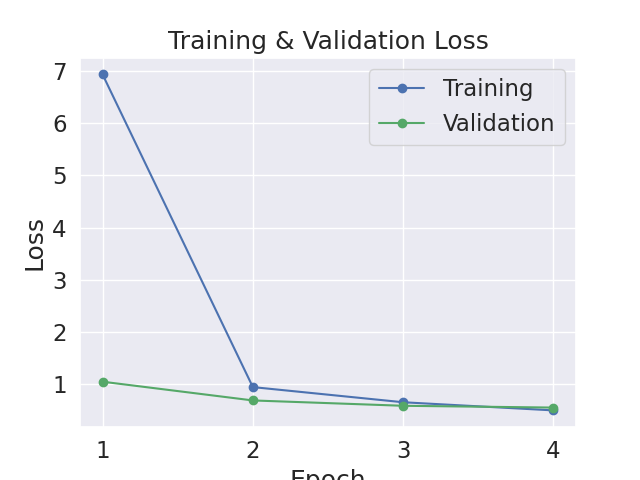
\includegraphics[width=0.4\textwidth]{\rootDir/stats/plot_gpt2_finetuning_weather_and_seasons.png}
        }    
    \end{figure}
    All implementation details are in src\slash utils\slash gpt2.py file. Each model is saved in models\slash gpt2\slash label folder.

    \subsection{Generating Tweets}\label{sec:generating-tweets}
    If we fine tune gpt2-fa on politics label amd we give it prompt about politics, we expect it to generate a tweet about politics. The following image shows the result of this experiment.
    \begin{center}
        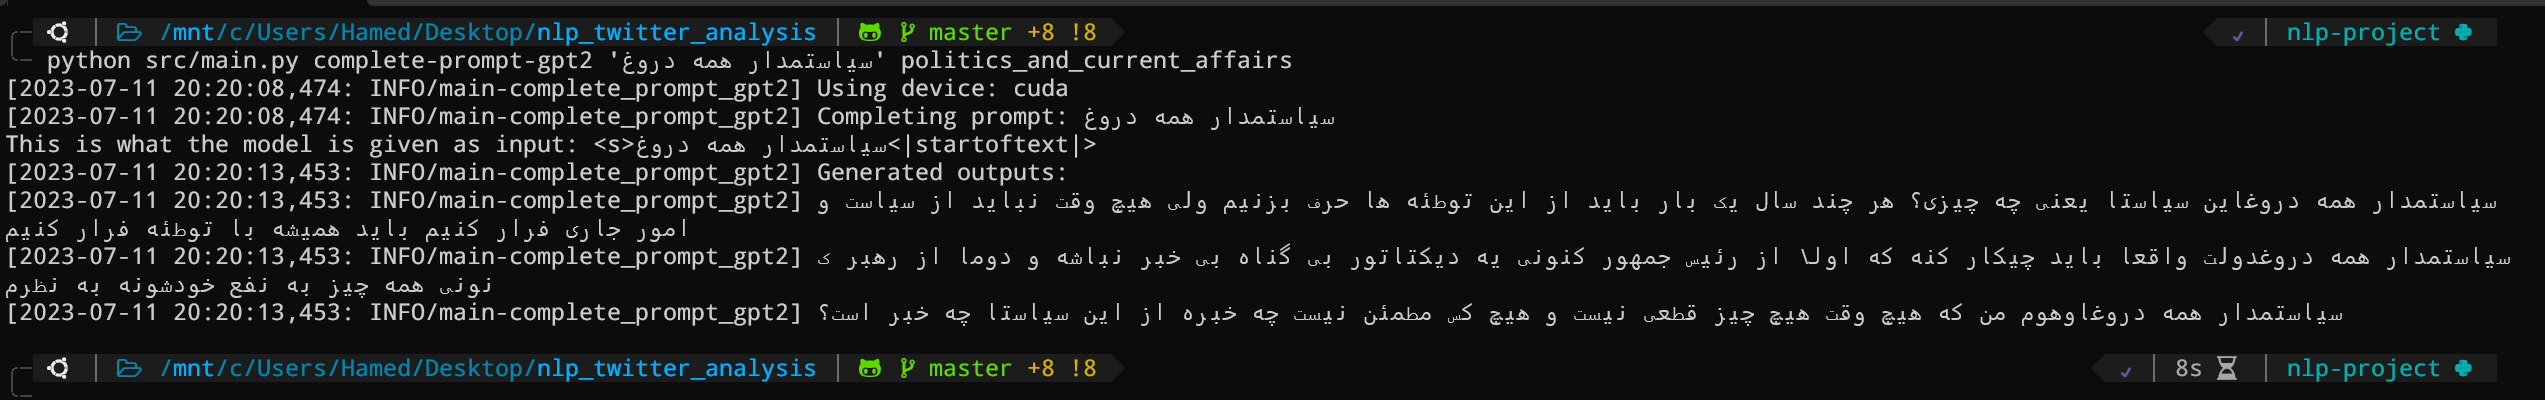
\includegraphics[width=1\textwidth]{\rootDir/src/latex/images/gpt2_generation.png}
    \end{center}
    It is important to note that we should set max\_seq length according to the common length of the tweets in the dataset. If we set it a large number, then model will be overfitted on PAD token and it will generate a lot of PAD tokens.

    \section{Resources}\label{sec:resources}
    \begin{itemize}
        \item \url{https://github.com/hooshvare/parsgpt}
        \item \url{}
    \end{itemize}

\end{document}
